% calibration of heo /mnt/backup/safe-with-time/torben/safed/y2009/0512
% measurement double plane /mnt/backup/safe-with-time/torben/safed/0525
\chapter{Holographic approach to spatio-angular illumination}


A system is constructed for doing angular and spatially controlled illumination. It is based on a phase only spatial light modulator that is used to steer a coherent laser beam.

\section{Introduction}
In the MEMI project a system will be built that contains two separate
display devices (a micro mirror array (MMA) and a ferroelectric liquid
crystal on silicon display (FLCOS)). Both of these displays have to be
used in a pulsed mode. The FLCOS is driven with a 2kHz alternating
voltage and a lot of care is taken that the duty cycle is exactly 50\%
as a net current would destroy the liquid crystal cell. The voltage
that tilts the MMA mirrors is stored as a charge in capacitors on its
CMOS backplane. The capacitors discharge over time. To maintain a
constant angle the mirrors have to be constantly refreshed.

In this report we describe a very different approach that simplifies
the setup considerably.

\includegraphics[width=12cm]{holo-setup}

The above image shows a sketch of the setup. A holographic grating is
positioned in the intermediate image plane. First consider what
happens if we replace the grating with a mirror: the reflected
(zero-order) light won't reach the objective as it is blocked in the
back focal plane.

\section{Description of the holographic method}
The direction and periodicity of a holographic blazed grating can now
be chosen so, that the first order is steered into any position on the
back focal plane. In the sketch the grating directs the first order
into the centre of the back focal plane. Accordingly the region that
contains the (demagnified) grating will be illuminated with parallel
light. Decreasing the size of the grating will decrease the size of
the illuminated area in the object. Note that a grating of very small
size will make a broad order in the back focal plane, limiting the
possible angular control.
\section{Description of the experimental setup}
We use a HEO 1080 P High-Resolution LCOS Phase Only Spatial Light
Modulator (Holoeye, Berlin, Germany) to control the phase in the
intermediate plane. The illumination is a 473 nm diode laser. It is
coupled into a polarization maintaining fiber and collimated by a 150
mm lens with 50 mm diameter.

The tube lens has 300 mm diameter and the objective is a 63x/NA 1.4
with oil immersion.  For aligning the optical system a sequence of
device filling gratings was displayed at 60Hz. The parameters of the
grating were chosen so that the point describes a circle in the back
focal plane. It was then possible to align the LCOS angle so that the
parallel beams leave the objective at the same angle relative to the
optical axis.

\section{Description of the sample}
To show that the illumination angle of the light was indeed adjustable
a special sample was constructed. A slide and a cover slip were coated
with a thin layer of fluorophore. The air gap between was
approximately five micrometers.

Imaging the fluorphore plane on the slide resulted in a haze of
background fluorescence stemming from the cover slip. Changing the
illumination angle resulted in a rotation of this haze as one would
expect. The numbers in the following image are the azimuth of the
illumination angle in degree.

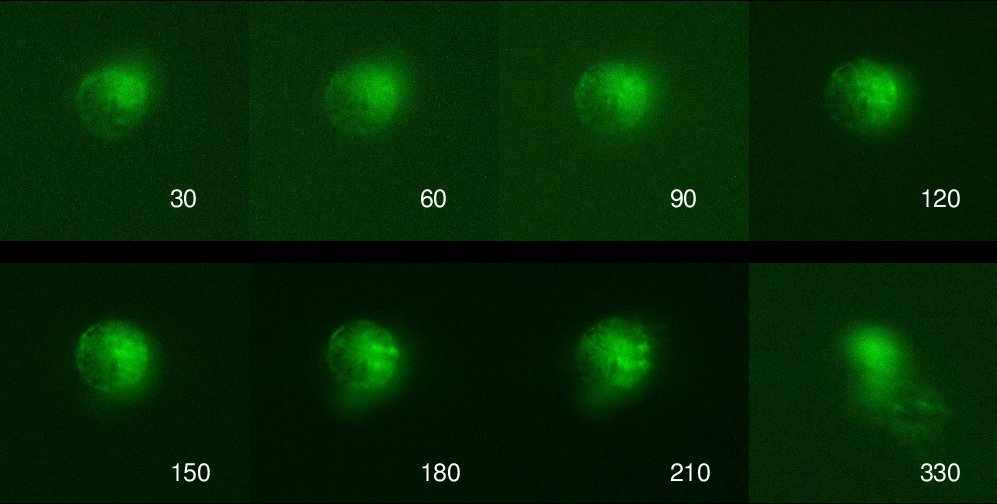
\includegraphics[width=12cm]{haze}

\section{Conclusion}
With our prototype system we showed that it is feasible to use the
phase only SLM to do angular and spatial illumination. Further work
would be necessary to optimize the grating fine structure so that more
light is directed towards the first order (blazing). Compared to the
MEMI system a lot less synchronization issues are involved. But note
that this technique is only possible with coherent
illumination. Furthermore there is no inherent advantage in the method
that is described in this report as light from dark areas is sent into
a beam stop as in the MEMI system.

Its probably possible to build a system using a kinoform element (two
phase holograms in different positions). This would allow to redirect
light from dark areas into bright areas leading to a much more
efficient system.

\section{ Characterization of phase-only spatial light modulator}
\section{Introduction}
\label{sec-1}

I measure the correspondance between gray values and phase difference
on the Holoeye HEO 1080P spatial light modulator. I use approximately
the same setup as given in the Manual (page 9/13, Application Note,
HDTV Phase Panel Devloper Kit, rev 4, 5. May 2006). A sketch of the
setup is shown in the following figure:

\centerline{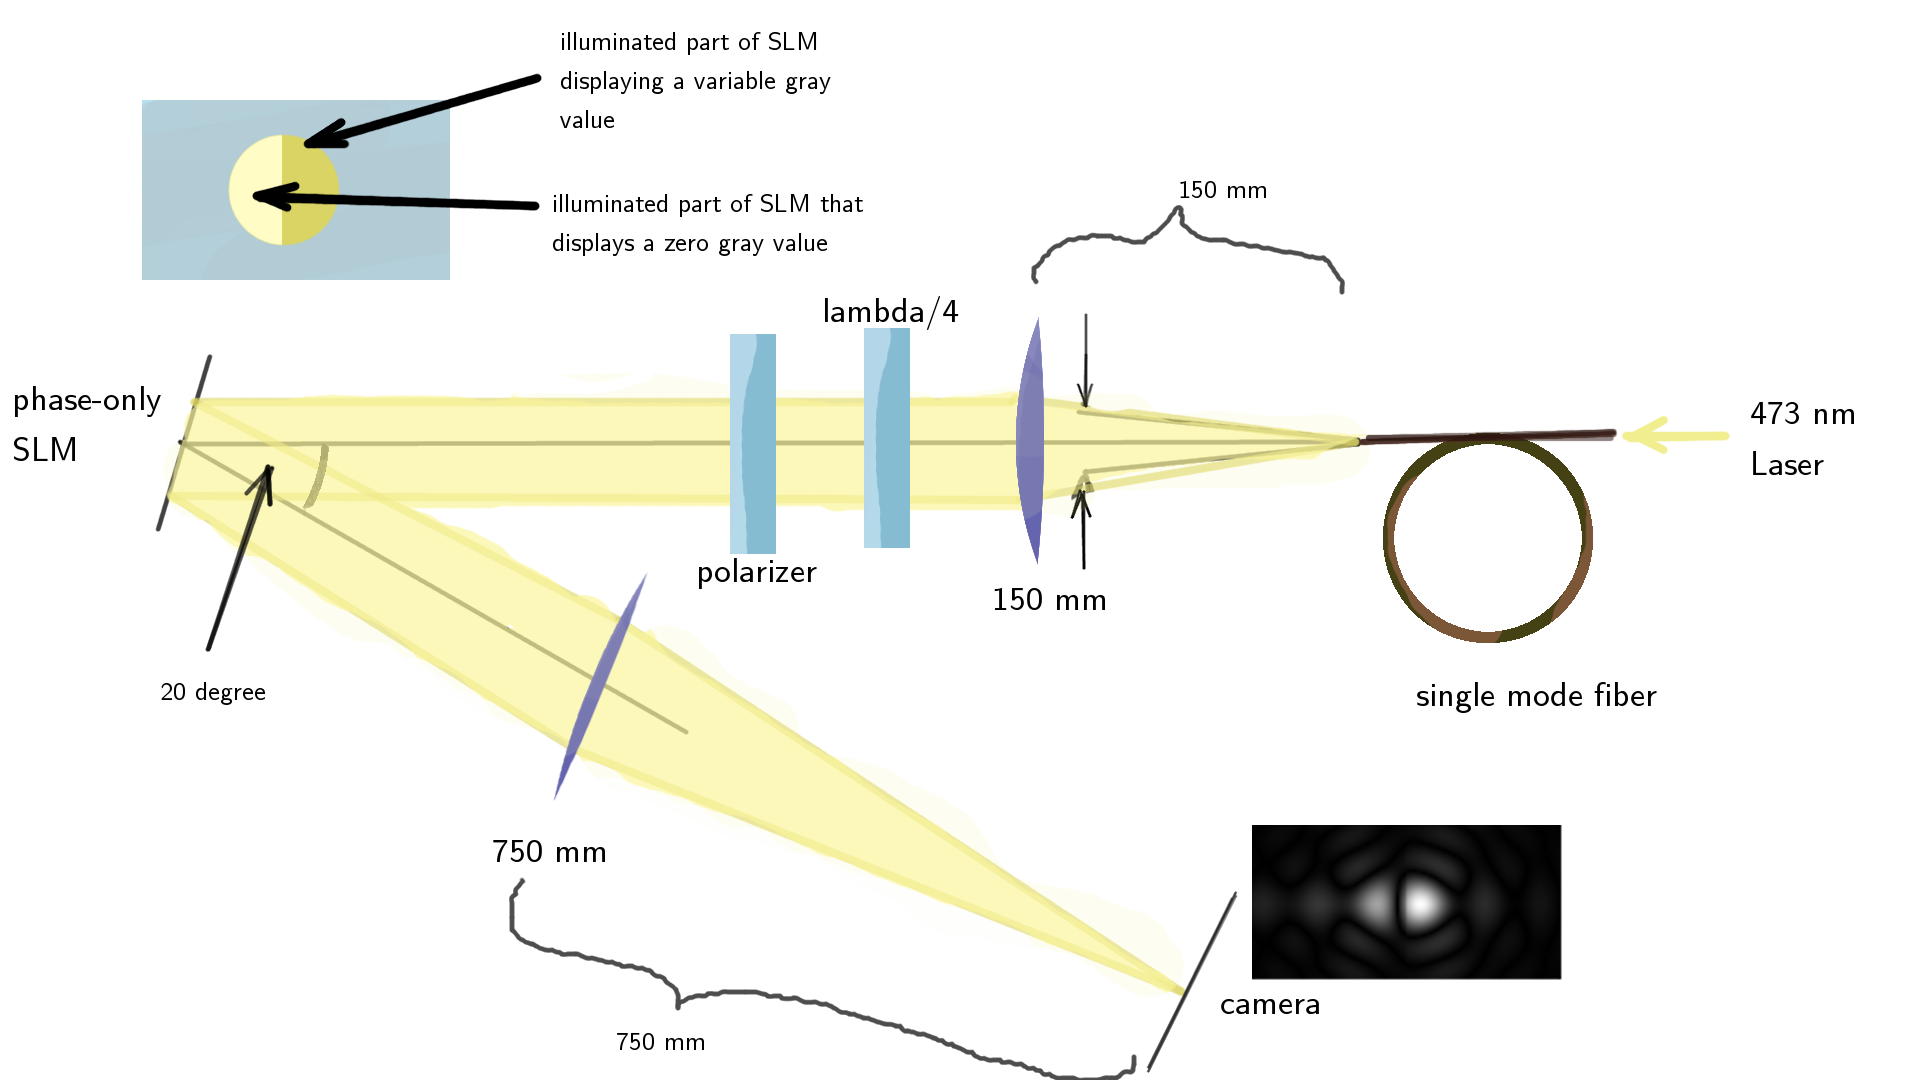
\includegraphics[width=16cm]{sketch}}


The SLM is illuminated with a plane linear polarized wave. The plane
of polarization lies in the paper plane. The orientation of the SLM is
such that the cable comes out on the top of the device (perpendicular to
paper plane).

The SLM displays two vertical bars. The left bar (in the bottom of the
sketch) shows black and the upper bar displays a gray value that is
varyied for the measurement.
The beam has a circular shape and a (sufficiently) constant intensity
distribution. The beam is centered on the line between the two bars
of different phase.
In contrast to the measurement setup in the manual I did not put an
analyzer in front of the camera.

\section{Numerical simulation}
\label{sec-2}

Another difference of my setup is that I don't employ a mask to get
two circular beams on the SLM. However minima of the diffraction
pattern in the fourier plane (on the camera) still move proportional
to the phase difference between the two beams as the following
simulation proves:


\centerline{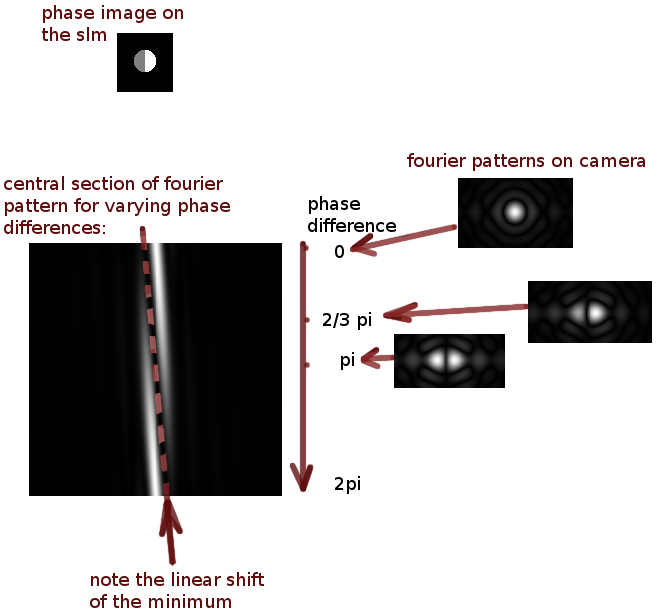
\includegraphics[width=12cm]{theory}}


For the simulation I calculated the Fourier transform of a phase image
with a geometry as shown in the top left picture.  The three images on
the right show the Fraunhofer diffraction patterns of this
(reflective) phase image for three different values of the phase
difference between the half circles. The position of the minimum
changes proportionally to the phase difference. So I can measure the
position of the extrema to do determine the relationship between gray
value and phase difference.

\section{Measurement}
\label{sec-3}


The result of this measurement (horizontal section through center of
the Fourier pattern against gray value) is shown in the top of the
following figure.

\centerline{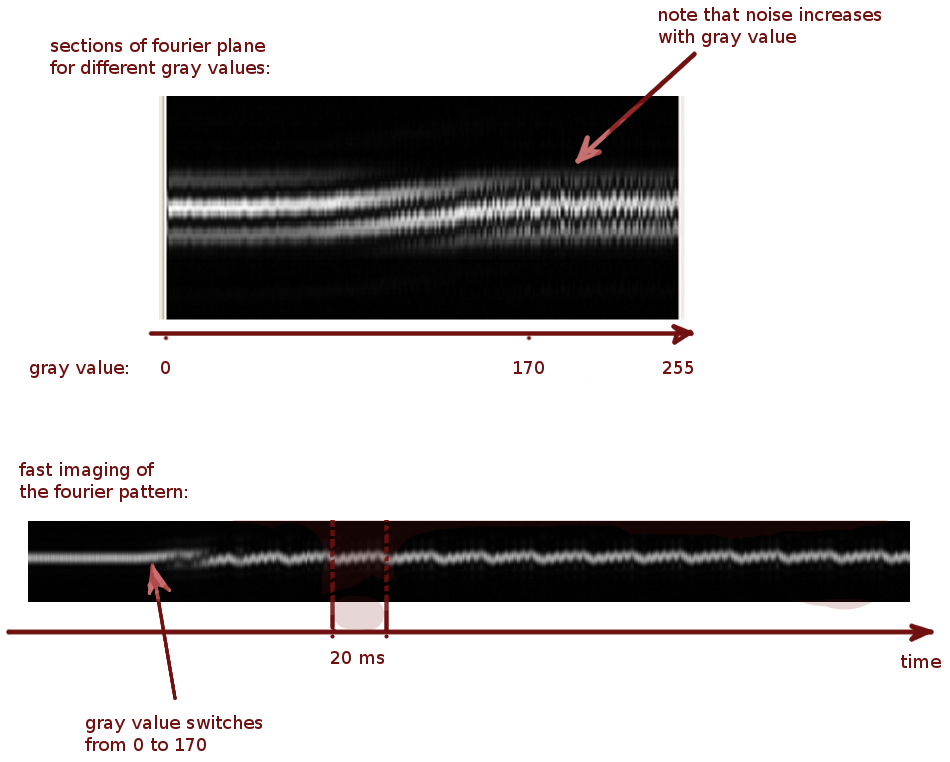
\includegraphics[width=16cm]{measure}}


The measurement shows that a phase difference of $2\pi$ can be induced
for a sufficiently high gray value. However for the top image shows
significant noise. There are jumps in the data that amount to several
10 gray values. As it turns out this isn't noise but the phase
difference is time dependent.

To analyse this effect further a fast camera (mvBlueFox 102G, 2400 Hz,
$200\times4$ region of interest, $\unit[ 6]{\mu m}$ pixel size) was
used to image the Fourier pattern with a high time resolution.  The
bottom image displays 1000 horizontal line sections over center of the
Fourier plane. In the beginning both half circles were displaying a
gray value of zero. Then the right half circle was suddenly set
to 170. The transient occurs quite fast but then there is a waveform
with 5 peaks that repeats with 50 Hz (the refresh rate of the
display).


\section{Conclusion}
\label{sec-4}

The measurement suggests that the phase difference of the Holoeye SLM
is varying significantly over time. In order to improve the
performance for displaying computer generated holograms it will be
necessary to employ a pulsed laser source that is flashing in sync with
the video frame rate.

